\documentclass[10pt,a4paper]{article}

\usepackage[utf8x]{inputenc}
\usepackage[english]{babel}
\usepackage[T1]{fontenc,url}
\usepackage[hang,small,bf]{caption}
\usepackage{relsize}
\usepackage{setspace}
\usepackage{parskip}
\usepackage{lmodern}
\usepackage{microtype}
\usepackage{verbatim}
\usepackage{amsmath, amssymb, amsthm}
\usepackage{mathtools}
\usepackage{tikz}
\usepackage{physics}
\usepackage{algorithm}
\usepackage{algpseudocode}
\usepackage{listings}
\usepackage{enumerate}
\usepackage{graphicx}
\usepackage{float}
\usepackage{hyperref}
\usepackage{varioref}
\usepackage{siunitx}
\usepackage{todonotes}
\usepackage{color}
\usepackage[margin=3cm]{geometry}
\labelformat{equation}{equation~(#1)}

\renewcommand{\exp}{\mathrm{e}^}
\newcommand{\halflife}{t_{\frac{1}{2}}}
\newcommand{\half}{\frac{1}{2}}
\newcommand{\planck}{$h = \SI{6.626e-34}{J.s}$}

\definecolor{light_green}{rgb}{0, 0.6, 0}
\definecolor{light_grey}{rgb}{0.5, 0.5, 0.5}
\definecolor{magenta}{rgb}{0.7, 0, 0.5}


\lstdefinestyle{py}{
    language = python,
    frame = single,
    showstringspaces = false,
    basicstyle = \small\ttfamily,
    breaklines = true,
    commentstyle = \color{light_grey},
    keywordstyle = \color{magenta},
    stringstyle = \color{light_green},
}


\begin{document}


\section*{Exercise E.1 - Boiling water}
\addcontentsline{toc}{section}{Exercise E.1 - Boiling water - \texttt{boiling\_water.py}}

Newton's law of cooling tells us how the temperature $T(t)$ to an object changes over $t$ minutes. 
It is formulated as such:
\[
\dv{T(t)}{t} = -k\qty(T(t) - T_e )
\]
where $T_e $ is the temperature to the environment and $k$ is the rate of change in temperature of the water. 

We will look closer at how the temperature to water at $15\,\si{\celsius}$ changes when being boiled in an old and worn out kettle. We will use Newton's law of cooling as a simple  model to the change of temperature.

At $t = 0$, we have that $T(0) = 15\,\si{\celsius}$. Also, let $k = 0.2$.

\subsection*{a)}
The kettle gets a temperature of $100\, \si{\celsius}$ immediately after being turned on. In other words, we have that  $T_e = 100\,\si{\celsius}$  for all values of $t$. 

Write a program which use \texttt{ODESolver} to calculate the temperature of the water $T(t)$. Use $N = 1000$ uniformly distributed values for $t$ between 0 and 15.
\subsection*{b)}
As you probably saw in a) it takes the kettle long time to make the water reach $100\,\si{\celsius}$. A friend of yours tries to fix your kettle, but unluckily manages to make it worse. You make some measurements to see how badly the kettle has become, and notices that the temperature of the kettle varies according to the following model:
\[
T_e(t) = 20\sin\qty(\frac{\pi}{3}t)+80
\]

Extend your program from a) such that it finds the temperature $T(t)$ of the water in the broken kettle.

Let your program plot the temperature $T$ of the water from a) along with the temperature $T$ your program finds in this subtask. 

Filename: \texttt{boiling\_water.py}






\section*{Exercise E.2 - RC circuit}
\addcontentsline{toc}{section}{Exercise E.2 - RC circuit - \texttt{RC.py}}
The object of this exercise is to study the change in electric charge $Q$ held by a capacitor over time. 

Figure \ref{fig:E2_RC} shows an RC-circuit, containing a capacitor, a resistor and a battery (voltage source). Our focus will be on the capacitor, which consists of two parallel metal plates. When a voltage source is connected, the metal plates gets charged with positive and negative electric charges. When the voltage source is disconnected, the electric charges flows back through the circuit in opposite direction, until the capacitor is entirely discharged, and $Q = \SI{0}{C}$.


\begin{center}
	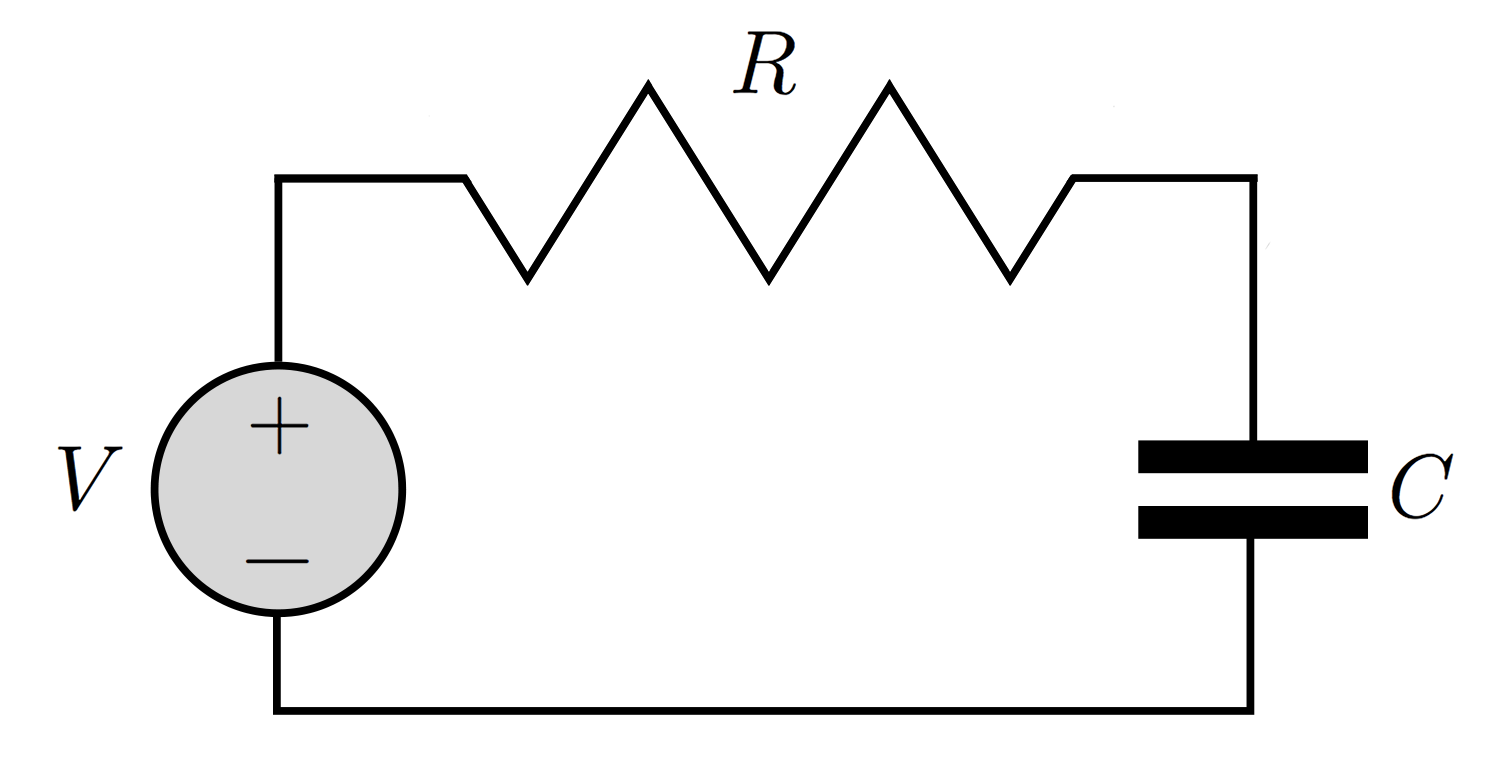
\includegraphics[scale=1]{fig_RC-cp1.png}
	\captionof{figure}{Illustration of a RC-circuit.}
    \label{fig:E2_RC}
\end{center}

The battery provides a constant voltage $V$ (measured in Volt) when turned on. The resistors resistance is given as $R$ (in Ohm), and tells how well it blocks electric current. The capacitor has a capacitance $C$ (in Farad), which tells how well it can hold electric charge.

The amount of electric charge the capacitor holds at a certain time is given by differential equation
\begin{align}\label{eqn:Qder}
Q'(t) = \frac{V}{R} - Q(t)\frac{1}{RC}
\end{align}

\subsection*{a)}
Use ODESolver to solve for $Q(t)$ over the first 10 seconds with 101 timesteps. Set the battery's voltage to $V = \SI{8}{Volt}$, the capacitors capacitance to $C = \SI{2e-8}{Farad}$, and the resistors resistance to $R = \SI{e8}{Ohm}$. The capacitor has no charge, $Q_0=0$, at $t=0$. Use both Forward Euler and Runge Kutta 4, and plot both results together with the analytical solution
\begin{align}
Q(t) = (Q_0 - CV)\exp{-t/RC} + CV
\end{align}

Reduce the number of timesteps until you can visibly distinguish both numerical methods from the exact solution.


\subsection*{b)}
The battery becomes unstable at $t=\SI{10}{s}$, and the voltage starts oscillating as a sinus wave. At $t = \SI{20}{s}$ the battery breaks completely. We can implement this by making the voltage a variable of time, $V(t)$. We are still solving the differential $\ref{eqn:Qder}$, but now with a voltage given as
\begin{equation}
V(t) =
\begin{cases}
    8,           &t < 10 \\
    4\sin(t)+4,  &10 < t < 20 \\
    0,           &t > 20
\end{cases}
\end{equation}

Plot the new solution, $Q(t)$ over 30 seconds with Runge Kutta 4 and 101 timepoints. 

Filename: \texttt{RC.py}



\section*{Exercise E.3 - Throwing ball with air resistance}
\addcontentsline{toc}{section}{Exercise E.3 - Throwing ball with air resistance - \texttt{throw\_air\_resistance.py}}
In this task we will simulate a ball being thrown where we include air resistance. To do so, we will use \texttt{ODESolver.py}.

The wind moves in the same direction as the ball is being thrown. 

We must solve the following equations to find the position of the ball:
\begin{align*}
\dv{x}{t} &= v_x \\
\dv{v_x}{t} &= -\frac{1}{2m}\rho C \pi R^2 \qty(v_x - w)^2 \\
\hfill \\
\dv{y}{t} &= v_y \\
\dv{v_y}{t} &= -g
\end{align*}
where $C = 0.47$ is a measurement on how much resistance the ball does at the air, $R$ is the radius of the ball, $m$ is the mass of the ball, $v_x$ is the velocity of the ball along the x-axis, $w$ the velocity of the wind and $g = 9.81\,\si{\meter.\per\square\second}$.

The initial conditions for this model are:
\begin{align*} 
x(0) &= 0 \\
v_x(0) &= v_0\cos\theta
\hfill \\
y(0) &= 0 \\
v_y(0) &= v_0\sin\theta
\end{align*}
where $\theta$ is the angle and $v_0$ the velocity (in \si{\meter.\per\second}) the ball was thrown with. 

\subsection*{a)}
Define a class which contains information about this problem. The class must have the same structure as the class \texttt{Problem} at page 790 in the book (or page 745 is you use the 4th edition). \\
The class in this exercise must have a constructor which takes in the initial conditions as a list, the radius $R$ of the ball, the mass $m$ of the ball and the velocity of the wind $w$. 

The class must also contain a \texttt{\_\_call\_\_}-function which returns the list: 
\begin{center}
\texttt{[vx,$ -\dfrac{1}{2m}\rho C \pi R^2 \qty(v_x - w)^2$,vy,$-g$]}  
\end{center}
where \texttt{vx} and \texttt{vy} is found in the same matter at page 790 in the book (or 745). 
\subsection*{b)} 
We will now see how the velocity of the wind affects the motion of the ball over $T = \SI{0.5}{\second}$. 

Assume that someone throw a ball with radius $R = 0.03275\,\si{\meter}$ and mass $m = 0.057\,\si{\kg}$ with an angle $\theta = \frac{\pi}{4}$ and velocity $ v_0 = 10 \,\si{\meter.\per\second}$. Also, let  $x(0) = 0$ and $y(0) = 0$.

We will look at the velocities of the wind $w = -10,-5,0,5,\text{ og }10$.
For every velocity $w$, the program must do the following:
\begin{itemize}
	\item[1)] Initialize and instance of the class defined a) where the values of r $R$,$m$, $w$ and list of initial conditions is sent as parameters to the constructor. The list of initial conditions \texttt{U0} might have the following structure:
	
	\texttt{U0} = \texttt{[x0, vx0, y0, vy0]} 
	
	where \texttt{x0} = $x(0)$, \texttt{vx0} = $v_0\cos\qty(\theta)$, \texttt{y0} = $y(0)$ og \texttt{vy0} = $v_0\sin\qty(\theta)$. 
	
	\item[2)] Let \texttt{ODESolver} find the positions. You are free to choose which numerical method \texttt{ODESolver}  should use to solve the ODEs. Be aware to send enough timepoints to the function \texttt{solve} from \texttt{ODEsolver} such that you get reasonable results. 
	
	\item[3)] Send the found positions from step 2) to \texttt{plt.plot(x,y)}. Be aware to get the correct values from the matrix \texttt{solve} from \texttt{ODESolver} returns!
\end{itemize}
When your program has finished the above steps for every $w$, let your program call \texttt{plt.show()} to display the motion of the ball for every value fo $w$. 


\textbf{Important: } When you have to plot several graphs in one plot, it is very important to be able to distinguish them somehow. To do so, one could use a list of strings which describes what is unique for every graph. The list can so be sent to \texttt{plt.legend} \textit{before} \texttt{plt.show()}  has been called. For instance, in our case we can do the following: 

\lstinputlisting[style=py]{pseudo_E3.py}

to be able to determine which graph corresponds to which velocity $w$ of the wind. 

Filename: \texttt{throw\_air\_resistance.py}




\section*{Exercise E.4 - Planetary orbits}
\addcontentsline{toc}{section}{Exercise E.4 - Planetary orbits - \texttt{Orbits.py}}

In this exercise we will study the orbit of the earth around the sun with 2nd order ODEs. Because the earth revolves around the sun in a plane, we can model its movement in only two dimensions, which we'll call $x$ and $y$.

Newtons gravitational law tells us the gravitational force between two objects. If we decompose this law into the $x$ and $y$ direction, and inserts it into Newtons second law, we can solve for the acceleration of Earth:
\begin{align}
\frac{d^2x}{dt^2} = -G\frac{M_{sun}x}{x^2+y^2} \quad\quad\quad\quad \frac{d^2y}{dt^2} = -G\frac{M_{sun}y}{x^2+y^2}
\label{eqn:E4}
\end{align}
Here, $M_{sun}$ is the mass of the sun, $G$ is the gravitational constant, and $x$ and $y$ is the distance from the Sun in $x$ and $y$ directions.

We will in this exercise use astronomical units instead of SI units, meaning that we will
\begin{itemize}
\item measure time in years (yr) instead of seconds.
\item measure distances in Astronomical Units (AU) instead of meters.\footnote{1 AU is the average distance between the Sun and Earth} 
\item measure masses in Solar Masses (SM) instead of kilograms.
\end{itemize}
This has the effect that
\begin{itemize}
\item the gravitational constant becomes $G = 4\pi^2\si{AU^3.yr^{-2}.SM^{-1}}$.
\item the mass of the Sun is $M_{sun} = \SI{1}{SM}$.
\item the initial position of Earth can be set to $x = \SI{1}{AU}$, $y = \SI{0}{AU}$.
\item the initial velocity of Earth can be set to $v_x = \SI{0}{AU/yr}$, $v_y = \SI{2\pi}{AU/yr}$.
\end{itemize}

Use the \texttt{ODESolver} to solve for the movement of the Earth around the Sun for 10 years using \ref{eqn:E4} and the initial conditions and parameters described above.\\
For more information on how to set up 2nd order ODEs, see the book, page 799-801.

Plot $y$ against $x$ for the 10 years, and you should observe a circular orbit of the earth around the origin, in a distance $\SI{1}{AU}$.

\textbf{Hint:} Matplotlib doesn't keep axis aligned by default, and circular orbits may look elliptical. You can change this by setting \texttt{matplotlib.pyplot.axis('equal')}

Filename: \texttt{Orbits.py}



















\end{document}
